\documentclass[fleqn]{beamer}
\usetheme{CambridgeUK}
\usepackage{tikz}
\usetikzlibrary{arrows}
\usepackage{amsmath}
\usepackage{amssymb}
\usefonttheme[onlymath]{serif}
\usepackage{pgfplots}
\usepackage{fancybox}
\usepackage{listings}
\setbeamerfont{frametitle}{size=\normalsize}
\setbeamerfont{framesubtitle}{size=\normalsize}
\setbeamertemplate{footline}[frame number]

\newcommand{\bs}[1]{\boldsymbol{#1}}

\title{New Approaches for Adjoint-Based
Error Estimation and Mesh Adaptation in
Stabilized Finite Element Methods with an
Emphasis on Solid Mechanics Applications}
\date{January, 2018}
\author{Brian N. Granzow}
\institute{
Mechanical Engineering\\
Rensselaer Polytechnic Instutite\\
Troy, NY 12180 USA}

\begin{document}

\setbeamercolor{background canvas}{bg=white}
\beamertemplatenavigationsymbolsempty

%==============================================================================

%% TITLE SLIDE
\begin{frame}
\titlepage
\begin{center}
\includegraphics[width=0.15\textwidth]{../img/rpi_seal}
\end{center}
\end{frame}

%==============================================================================

%% ABOUT THIS TALK
\begin{frame}{About this talk}
\begin{itemize}
\item Review of adjoint-based \emph{a posteriori} error estimation.
\item An automated approach for adjoint-based analysis.
\item Example applications of the automated approach.
\item A non-uniform refinement approach for adjoint analysis.
\item Goal-oriented analysis for variational multiscale methods.
\item Summary and conclusions.
\end{itemize}
\end{frame}

%==============================================================================

%% ERROR ESTIMATION
\begin{frame}{Adjoint-based \emph{a posteriori} error estimation}
{Error estimation}
The big picture:
\begin{itemize}
\item Partial Differential equation (PDE) $\rightarrow$ exact solution $u$.
\item PDE $\rightarrow$ analytic solution $u$ is, in general, unknown.
\item Finite Element Method (FEM) $\rightarrow$ approx. PDE solution $u^H$.
\item FEM $\rightarrow$ error associated with the discretization, $e := u-u^H$.
\item Analyst $\rightarrow$ how reliable/accurate is the solution $u^H$?
\end{itemize}
\end{frame}

%==============================================================================

% A POSTERIORI ERROR
\begin{frame}{Adjoint-based \emph{a posteriori} error estimation}
{\emph{A posteriori} error estimation}
Provides a useful analysis tool to:
\begin{itemize}
\item measure the accuracy of FEM approximations $u^H$.
\item control errors in FEM approximations (e.g. mesh adaptation).
\end{itemize}
Traditional estimates:
\begin{itemize}
\item choose a norm: $\| \cdot \|$ (e.g. energy, $L_2$)
\item approximate: $\mathcal{E} \approx \| e \|$.
\end{itemize}
Goal-oriented error estimates:
\begin{itemize}
\item choose a physically meaningful functional: $J(u)$.
\item approximate: $\mathcal{E} \approx J(u) - J(u^H)$.
\end{itemize}
\end{frame}

%==============================================================================

%% HIGH LEVEL STEPS
\begin{frame}{Adjoint-based \emph{a posteriori} error estimation}
{High level steps}
From a high level, adjoint-based error analysis follows the steps:
\begin{itemize}
\item Choose a physically meaningful functional quantity $J(u)$.
\item Solve the PDE of interest approximately with the FEM $\rightarrow u^H$.
\item Solve an auxiliary adjoint PDE with the FEM $\rightarrow z^H$.
\item Determine an enriched representation of the dual solution $z^h$.
\item Utilize $u^H$, $z^H$, and $z^h$ to estimate $J(u) - J(u^H)$.
\item Localize contributions to $J(u) - J(u^H)$ to mesh entities.
\item Use localized error contributions to drive adaptation.
\end{itemize}
Key features:
\begin{itemize}
\item The adjoint PDE relates $J(u)$ to the original PDE of interest.
\item $z \rightarrow$ sensitivity of the functional quantity of
interest with respect to perturbations in the original PDE residual.
\end{itemize}
\end{frame}

%==============================================================================

%%% MATHEMATICAL FOUNDATION
\begin{frame}{Adjoint-based \emph{a posteriori} error estimation}
{Mathematical foundation}
\scriptsize
\begin{equation*}
\hspace*{-3em}
\begin{aligned}
{\color{blue} Primal} \quad &
\boxed{
\text{Find} \; u \in V \; \text{such that} \; R_g(w;u) = 0
\quad \forall w \in V
} \\
{\color{blue} FEM} \quad &
\boxed{
\text{Find} \; u^H \in V^H \; \text{such that} \; R_g(w^H; u^H) 
+ R_{\tau}(w^H; u^H) = 0
\quad \forall w^H \in V^H
} \\
{\color{blue} Dual} \quad &
\boxed{
\text{Find} \; z \in V \; \text{such that} \; R'_g[u^H](w, z) =  J'[u^H](w)
\quad \forall w \in V
} \\
{\color{blue} Error} \quad &
\boxed{
J(u) - J(u^H) =
\underbrace{-R_g(z - z^H; u^H) + R_{\tau}(z^H; u^H)}_{\text{discretization error}} +
\underbrace{\mathcal{O}(e^2)}_{\text{linearization error}}
\forall w^H \in V^H
}
\end{aligned}
\end{equation*}

\begin{itemize}
\item $J'[u^H](w)$ - Fr\'{e}chet linearization about $u^H$.
\item $R'[u^H](w)$ - Fr\'{e}chet linearization about $u^H$.
\item Error representation obtained from functional relation to the
primal PDE residual via the dual solution $z$.
\end{itemize}
\end{frame}

%==============================================================================

%%% A TWO LEVEL APPROACH
\begin{frame}{Adjoint-based \emph{a posteriori} error estimation}
{A two-level approach}
\scriptsize

\begin{minipage}{.5\textwidth}
Two discretization levels: \\
$V^H \subset V \rightarrow$ coarse space \\
$V^h \subset V \rightarrow$  fine space \\ [8pt]
%
Primal equation discretized by FEM:
\begin{equation*}
\begin{aligned}
{\color{blue} Coarse} \quad & \boxed{ \bs{R}^H(\bs{u}^H) = \bs{0} } \\
{\color{blue} Fine} \quad & \boxed{ \bs{R}^h(\bs{u}^h) = \bs{0}} \\
\end{aligned}
\end{equation*}
%
$\bs{R}^H : \mathbb{R}^N \to \mathbb{R}^N$ \\
$\bs{R}^h : \mathbb{R}^n \to \mathbb{R}^n$ \\ [8pt]
%
Functional discretized by FEM: \\
$J^H : \mathbb{R}^N \to \mathbb{R}$ \\
$J^h : \mathbb{R}^n \to \mathbb{R}$ \\
\end{minipage}%
\begin{minipage}{0.5\textwidth}
%
Let $\bs{u}^h_H : I^h_H \bs{u}^H$ be prolongation of $u^H$
onto the fine space $V^h$, where $I^h_H : V^H \to V^H$. \\ [8pt]
Taylor expansions of fine space lead to:
%
\begin{equation*}
J^h(\bs{u}^h) - J^H(\bs{u}^H) \approx - \bs{z}^h \cdot \bs{R}^h(\bs{u}^h_H)
\end{equation*}
%
where $\bs{z}^h$ is the solution to the adjoint problem on
the fine space given by
%
\begin{equation*}
\left[ \frac{\partial \bs{R}^h}{\partial \bs{u}^h} \biggr|_{\bs{u}^h_H} \right]^T
\bs{z}^h =
\left[ \frac{\partial J^h}{\partial \bs{u}^h} \biggr|_{\bs{u}^h_H} \right]^T
\end{equation*}
\end{minipage}
\end{frame}

%==============================================================================

%%% MY CONTRIBUTIONS
\begin{frame}{Adjoint-based \emph{a posteriori} error estimation}
{My contributions}
\begin{itemize}
\item A fully automated approach for adjoint-based error estimation.
\item Applicable to stabilized finite element methods.
\item Runs in parallel for solid mechanics applications.
\item Applied to finite deformation solid mechanics.
\item With complex three dimensional geometries.
\item Non-uniform refinement approaches for adjoint solves.
\item New adjoint-based error estimation for VMS methods.
\end{itemize}
\end{frame}

%==============================================================================

%% ACCESSIBILITY
\begin{frame}{An automated approach to adjoint-based error estimation}
{Accessibility to engineering practitioners}
Potential difficulties in goal oriented error estimation and
mesh adaptation for modern engineers practitioners:
\begin{itemize}
\item Many components must be implemented
$\rightarrow$ primal analysis, dual analysis,
dual enrichment, error localization, mesh adaptation
\item Residuals and functionals can be highly nonlinear
$\rightarrow$ linearizations are required
\item Problems of interest necessitate parallel analysis
$\rightarrow$ scalable primal and dual mechanics analysis code
is required.
\item Fully unstructured parallel mesh adaptation
$\rightarrow$ requires performant software tools.
\end{itemize}
\end{frame}

%==============================================================================

%% A POTENTIAL SOLUTION
\begin{frame}{An automated approach to adjoint-based error estimation}
{A potential solution}
A solution: I wrote a goal-oriented analysis library:\\
\vspace{1em}
https://github.com/bgranzow/goal
\vspace{1em}

\begin{itemize}
\item Utilizes performant software components (Trilinos and PUMI)
\item Automates primal, dual, and error localization steps
\item Allows for rapid implementation of new physics / QoIs
\item Approach similar to Albany / Panzer (Sandia codes)
\end{itemize}
\end{frame}

%==============================================================================

%% TEMPLATE BASED GENERIC PROGRAMMING
\begin{frame}{An automated approach to adjoint-based error estimation}
{Template-based generic programming}
\begin{center}
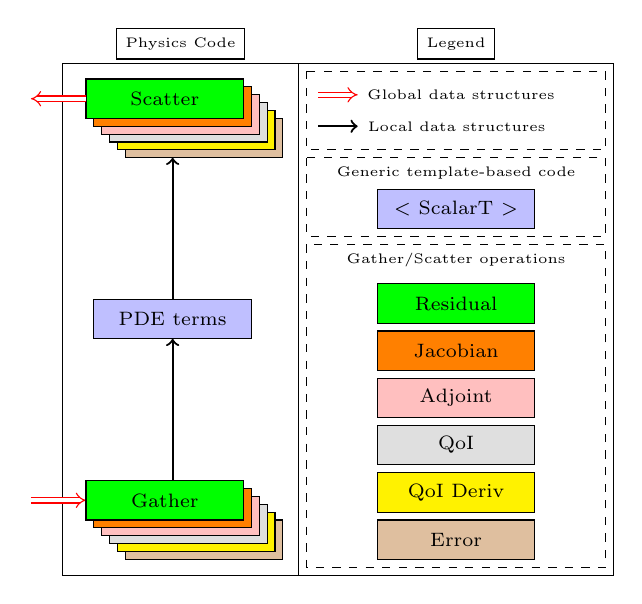
\begin{tikzpicture}

% physic code
\node[draw] at (1.5,6.25) {\tiny Physics Code};

% legend
\node[draw] at (5, 6.25) {\tiny Legend};

% bounding boxes
\draw (0,-0.5) rectangle +(3, 6.5);
\draw (3,-0.5) rectangle +(4, 6.5);

% global data transfer -> gather
\draw[red,-implies,double equal sign distance] (-0.4,0.45) -- (0.3,0.45);

% gather template operations
\draw[fill=brown!50] (0.8, -0.3) rectangle+(2,0.5);
\draw[fill=yellow] (0.7, -0.2) rectangle+(2,0.5);
\draw[fill=gray!25] (0.6, -0.1) rectangle+(2,0.5);
\draw[fill=pink] (0.5, 0.0) rectangle+(2,0.5);
\draw[fill=orange] (0.4, 0.1) rectangle+(2,0.5);
\draw[fill=green] (0.3, 0.2) rectangle +(2,0.5)
node[pos=0.5] {\scriptsize Gather};

% local data transfer gather -> pde
\draw[black,thick,->] (1.4,.7) -- (1.4,2.5);

% generic template pde evaluation
\draw[fill=blue!25] (0.4,2.5) rectangle +(2,0.5)
node[pos=0.5] {\scriptsize PDE terms};

% local data transfer pde -> scatter
\draw[black,thick,->] (1.4,3.0) -- (1.4,4.8);

% scatter template operations
\draw[fill=brown!50] (0.8, 5.3) rectangle+(2,-0.5);
\draw[fill=yellow] (0.7, 5.4) rectangle+(2,-0.5);
\draw[fill=gray!25] (0.6, 5.5) rectangle+(2,-0.5);
\draw[fill=pink] (0.5, 5.6) rectangle+(2,-0.5);
\draw[fill=orange] (0.4, 5.7) rectangle+(2,-0.5);
\draw[fill=green] (0.3, 5.8) rectangle+(2,-0.5)
node[pos=0.5] {\scriptsize Scatter};

% global data transfer <- scatter
\draw[red,implies-,double equal sign distance] (-0.4,5.55) -- (0.3,5.55);

% data transfer
\draw[dashed] (3.1,5.9) rectangle +(3.8,-1);
\draw[red,-implies,double equal sign distance] (3.25,5.6) -- (3.75,5.6)
node[black,anchor=west] {\tiny Global data structures};
\draw[black,thick,->] (3.25, 5.2) -- (3.75, 5.2)
node[black,anchor=west] {\tiny Local data structures};

% generic data evaluation type
\draw[dashed] (3.1, 4.8) rectangle +(3.8,-1);
\node[black] at (5,4.6) {\tiny Generic template-based code};
\draw[fill=blue!25] (4,4.4) rectangle +(2,-0.5)
node[pos=0.5] {\scriptsize $<$ ScalarT $>$};

% template specializations
\draw[dashed] (3.1, 3.7) rectangle +(3.8,-4.1);
\node[black] at (5,3.5) {\tiny Gather/Scatter operations};
\draw[fill=green] (4,3.2) rectangle +(2,-0.5)
node[pos=0.5] {\scriptsize Residual};
\draw[fill=orange] (4,2.6) rectangle +(2,-0.5)
node[pos=0.5] {\scriptsize Jacobian};
\draw[fill=pink] (4,2.0) rectangle +(2,-0.5)
node[pos=0.5] {\scriptsize Adjoint};
\draw[fill=gray!25] (4,1.4) rectangle +(2,-0.5)
node[pos=0.5] {\scriptsize QoI};
\draw[fill=yellow] (4,0.8) rectangle +(2,-0.5)
node[pos=0.5] {\scriptsize QoI Deriv};
\draw[fill=brown!50] (4,0.2) rectangle +(2,-0.5)
node[pos=0.5] {\scriptsize Error};
\end{tikzpicture}

\end{center}
\end{frame}

%==============================================================================

%% TEMPLATE SPECIALIZATION
\begin{frame}{An automated approach to adjoint-based error estimation}
{Evaluation purposes}
\scriptsize
\begin{itemize}
\item \fcolorbox{black}{green}{Residual} :
assembles residual vector, $R^H$
\item \fcolorbox{black}{orange}{Jacobian} :
assembles Jacobian matrix,
$\frac{\partial R^H}{\partial u^H}$
or adjoint $[\frac{\partial R^H}{\partial u^H} ]^T$
\item \fcolorbox{black}{pink}{QoI} :
computes functional, $J^H$, and assembles functional derivative,
$\frac{\partial J^H}{\partial u^H}$
\item \fcolorbox{black}{gray!25}{Error}
localizes error,
$\mathcal{E}_i = R_g((z^h - I^H z^h) \psi_i \; ; \; u^H) +
R_{\tau}((I^H z^h) \psi_i \; ; \; u^H)$
\end{itemize}

\begin{itemize}
\item Allows rapid implementation of new physics, quantities of interest
\item Avoids tedious / error-prone implementation of specialization-specific code.
\end{itemize}

\vspace{1em}
\hrule
\vspace{1em}
\scriptsize{
$\star$
Thomas Richter, and Thomas Wick.
\emph{Variational localizations of the dual weighted residual estimator}.
Journal of Computational and Applied Mathematics 279 (2015): 192-208.
}
\end{frame}

%==============================================================================

%% FINE SPACE
\begin{frame}{An automated approach to adjoint-based error estimation}
{Choice for the fine space}
%
\begin{minipage}{0.5\textwidth}
\begin{figure}
\includegraphics[width=0.99\textwidth]{../img/aut_glial_nested}
\end{figure}
\end{minipage}%
\begin{minipage}{0.5\textwidth}
\begin{itemize}
\item Global higher order solve $\rightarrow$ greater accuracy
\item Prefer over $p$-enrichment
\begin{itemize}
\item Stabilized FEM $\rightarrow$ higher order terms difficult to implement 
\item Higher order stabilized FEM $\rightarrow$ rarely used in practice
\end{itemize}
\end{itemize}
\end{minipage}
\end{frame}

%==============================================================================

%% EXAMPLE : BALANCE
\begin{frame}[containsverbatim]{An automated approach to adjoint-based error estimation}
{Balance of linear momentum residual}

\begin{lstlisting}[
language=C++,
directivestyle={\color{black}}
emph={int,char,double,float,unsigned},
emphstyle={\color{blue}},
basicstyle=\scriptsize,
frame = single,
]
for (int elem = 0; elem < workset.size; ++elem) {
  for (int ip = 0; ip < num_ips; ++ip)
  for (int node = 0; node < num_nodes; ++node)
  for (int i = 0; i < num_dims; ++i)
  for (int j = 0; j < num_dims; ++j)
    resid[i](elem, node, i) +=
      stress(elem, ip, i, j) *
      grad_w(elem, node, ip, i, j) *
      wdv(elem, ip);
}
\end{lstlisting}

\scriptsize
\begin{columns}
\begin{column}{0.5\textwidth}
Primal problem: involves:
\[
\frac{\partial {\color{red}R} ^H}{\partial u^H} \delta u^H= 
- {\color{red}R} ^H
\]
Dual problem: solve
\[
[ \frac{\partial {\color{red}R} ^h}{\partial u^h} ]^T z^h =
[\frac{\partial J^h}{\partial u^h} ]^T
\]
\end{column}
\begin{column}{0.5\textwidth}
Error localization:
\[
\hspace*{-6em}
\mathcal{E}_i = {\color{red}R}_g^h((z^h - I^H z^h) \psi_i \; ; \; u^H)
+ {\color{red}R}_{\tau}^h((I^H z^h) \psi_i \; ; \; u^H)
\]

\vspace{1em}

Key idea: \\
Evaluations share single implementation ${\color{red} R}$
\end{column}
\end{columns}

\end{frame}

%==============================================================================

%% CELL PROBLEM DEFINITION
\begin{frame}{Applications to finite deformation mechanics}
{A cell embedded in a matrix : problem definition}
\scriptsize
\begin{columns}
\begin{column}{0.5\textwidth}
\includegraphics[width=0.99\textwidth]{../img/mech_glial_geom} \\ [8pt]
Geometry for the cell problem
\vspace{1em}
\hrule
\vspace{1em}
Neohookean constitutive model: \\
$E = 600$ Pa \\
$\nu = 0.4999$ \\
$J(u) = \int_{\mathcal{B}_0} \frac13(u_x + u_y + u_z) \, \text{d} V$
\end{column}
\begin{column}{0.5\textwidth}%%
\includegraphics[width=0.99\textwidth]{../img/mech_glial_applied_traction} \\
Applied tractions for the cell problem
\includegraphics[width=0.99\textwidth]{../img/mech_glial_deformed} \\
Deformed cell membrane after tractions
\end{column}
\end{columns}
\end{frame}

%==============================================================================

%% CELL EFFECTIVITIES
\begin{frame}{Applications to finite deformation mechanics}
{A cell embedded in a matrix : parallelization}
Problem run with 16 MPI ranks \\
ParMA $\rightarrow$ load balancing to ensure partition quality \\
10 solve / adapt cycles for the model problem \\
\vspace{1em}
\begin{columns}
\begin{column}{0.5\textwidth}
\centering
\includegraphics[width=0.99\textwidth]{../img/aut_glial_initial_parts} \\
Initial mesh partitioning
\end{column}
\begin{column}{0.5\textwidth}%%
\centering
\includegraphics[width=0.99\textwidth]{../img/aut_glial_final_parts} \\
Final mesh partitioning
\end{column}
\end{columns}
\vspace{1em}
Reference QoI value $J(u) = −527.1453$ \\
using about $60$ million degrees of freedom
\end{frame}

%==============================================================================

%% CELL EFFECTIVITIES
\begin{frame}{Applications to finite deformation mechanics}
{A cell embedded in a matrix : effectivities}
\includegraphics[width=0.99\textwidth]{../img/mech_glial_effectivity_plot}
\end{frame}

%==============================================================================
%% CELL CONVERGENCE
\begin{frame}{Applications to finite deformation mechanics}
{A cell embedded in a matrix : error convergence}
\includegraphics[width=0.99\textwidth]{../img/mech_glial_convergence_plot}
\end{frame}

%==============================================================================

%% CELL MESHES
\begin{frame}{Applications to finite deformation mechanics}
{A cell embedded in a matrix : adapted meshes}
\begin{minipage}{0.5\textwidth}
\hspace*{-3em}
\includegraphics[width=1.3\textwidth]{../img/mech_glial_initial_mesh} \\
Initial mesh
\end{minipage}%
\begin{minipage}{0.5\textwidth}
\centering
\hspace*{-1em}
\includegraphics[width=1.3\textwidth]{../img/mech_glial_final_mesh} \\
Final adapted mesh
\end{minipage}
\end{frame}

%==============================================================================

%% SOLDER PROBLEM DEFINITION
\begin{frame}{Applications to finite deformation mechanics}
{Elastoplasticity in an array of solder joints : problem definition}
\scriptsize
\begin{minipage}{0.5\textwidth}
\begin{figure}
\centering
\includegraphics[width=0.95\textwidth]{../img/aut_solder_geom}
\end{figure}
Domain geometry problem geometry \\
\hrule
\vspace{1em}
$6 \times 6$ array of solder joints. \\
Between two dissimilar materials. \\
Cooled from $T_0 = 393K$ to $T_f = 318K$. \\ [8pt]
Elastoplastic constitutive model. \\
\vspace*{-1.25em}
\begin{itemize}
\item von-Mises yield criterion
\item Isotropic linear hardening
\item Thermal correction
\end{itemize}
\end{minipage}%
\begin{minipage}{0.5\textwidth}
\begin{figure}
\centering
\includegraphics[width=0.95\textwidth]{../img/aut_solder_qoi_geom}
\end{figure}
Solder joints defining the QoI \\ 
\hrule
\vspace{1em}
$J(u)$ : average von-Mises stress over $\mathcal{B}_0$. \\
$\mathcal{B}_0$ : defined by 3 solder joints \\
$\sigma_{vm} := \sqrt{\frac32 \bs{\sigma}' : \bs{\sigma}'}$ \\
$\bs{\sigma}'$ : deviatoric stress
\end{minipage}
\end{frame}

%==============================================================================

%% SOLDER WEAK SCALING
\begin{frame}{Applications to finite deformation mechanics}
{Elastoplasticity in an array of solder joints : weak scaling}
\begin{minipage}{0.6\textwidth}
\centering
\hspace*{-3.2em}
\includegraphics[width=1.15\textwidth]{../img/aut_weak_scaling}
\end{minipage}%
\begin{minipage}{0.4\textwidth}
Richardson extrapolation: \\
Reference value: \\
$J(u) = 328.9$ \\
\vspace{0.5em}
\hrule
\vspace{1em}
Final solve:
\begin{itemize}
\item 8192 MPI ranks
\item $> \frac12$ billion elements
\end{itemize}
\end{minipage}
\end{frame}

%==============================================================================

%% SOLDER ERROR
\begin{frame}{Applications to finite deformation mechanics}
{Elastoplasticity in an array of solder joints : errors}
\centering
\includegraphics[width=0.99\textwidth]{../img/aut_solder_error}
\end{frame}

%==============================================================================

%% SOLDER CONVERGENCE
\begin{frame}{Applications to finite deformation mechanics}
{Elastoplasticity in an array of solder joints : convergence}
$4 \times$ Solve primal $\rightarrow$ Solve adjoint $\rightarrow$ 
Estimate error $\rightarrow$ Adapt mesh \\
\vspace*{-1em}
\begin{center}
\includegraphics[width=0.8\textwidth]{../img/aut_solder_convergence}
\end{center}
\end{frame}

%==============================================================================

%% SOLDER ADAPTATION
\begin{frame}{Applications to finite deformation mechanics}
{Elastoplasticity in an array of solder joints : adaptation}
\centering
\includegraphics[width=0.7\textwidth]{../img/aut_solder_mesh_initial} \\
\includegraphics[width=0.7\textwidth]{../img/aut_solder_mesh_final}
\end{frame}

%==============================================================================

%% AUT SOLDER ADAPTATION 2
\begin{frame}{Applications to finite deformation mechanics}
{Elastoplasticity in an array of solder joints : adaptation}
\centering
\includegraphics[width=0.7\textwidth]{../img/aut_solder_mesh_initial2} \\
\includegraphics[width=0.7\textwidth]{../img/aut_solder_mesh_final2}
\end{frame}

%==============================================================================

%% REFINEMENT INTRO
\begin{frame}{Non-uniform refinement approaches for adjoint solves}
{Introduction}
Adjoint solution must be represented in richer FEM space \\
Full global enriched adjoint solve
\begin{itemize}
\item Guaranteed more accurate adjoint approximation
\item Expensive proposition
\end{itemize}
Reconstruction of adjoint problem in richer space
\begin{itemize}
\item More practical approach
\item Not guaranteed to yield more accurate adjoint
\end{itemize}
Compromise? Solve adjoint globally on non-uniformly refined meshes \\
\begin{itemize}
\item Less computationally expensive
\item Still maintains more accuracy in adjoint approximation
\end{itemize}
\end{frame}

%==============================================================================

%% LONG EDGE
\begin{frame}{Non-uniform refinement approaches for adjoint solves}
{Long edge refinement}
Mark longest edge in each element for refinement
\begin{minipage}{0.5\textwidth}
\centering
\includegraphics[width=0.99\textwidth]{../img/refine_long_mesh}
\end{minipage}%
\begin{minipage}{0.5\textwidth}
\centering
\includegraphics[width=0.99\textwidth]{../img/refine_long_mesh_3D}
\end{minipage}
\end{frame}

%==============================================================================

%% SINGLE EDGE
\begin{frame}{Non-uniform refinement approaches for adjoint solves}
{Single edge refinement}
Attempt to mark only a single edge in each element for refinement
\begin{minipage}{0.5\textwidth}
\centering
\includegraphics[width=0.99\textwidth]{../img/refine_single_mesh}
\end{minipage}%
\begin{minipage}{0.5\textwidth}
\centering
\includegraphics[width=0.99\textwidth]{../img/refine_single_mesh_3D}
\end{minipage}
\end{frame}

%==============================================================================

%% POISSON PROBLEM DEFINITION
\begin{frame}{Non-uniform refinement approaches for adjoint solves}
{Application to Poisson's equation}
\begin{minipage}{0.5\textwidth}
\centering
\includegraphics[width=0.99\textwidth]{../img/refine_squarehole_initial} \\
Initial mesh and point-wise QoI location for the Poisson example
problem
\end{minipage}%
\begin{minipage}{0.5\textwidth}
$R(w,u) := (\nabla w, \nabla u) - (w, f)$ \\ [8pt]
$f := 1$ \\ [8pt]
$J(u) := u(0.75, 0.75)$  \\ [8pt]
\hrule
\vspace{1em}
Compare adjoint-based error estimation when solving the adjoint
problem with meshes obtained with:
\begin{itemize}
\item Uniform refinement
\item Long-edge refinement
\item Single-edge refinement
\end{itemize}
\end{minipage}
\end{frame}

%==============================================================================

%% POISSON EFFECTIVIES
\begin{frame}{Non-uniform refinement approaches for adjoint solves}
{Application to Poisson's equation : effectivities}
\centering
\includegraphics[width=0.9\textwidth]{../img/refine_poisson_effectivity}
\end{frame}

%==============================================================================

%% POISSON DOFS
\begin{frame}{Non-uniform refinement approaches for adjoint solves}
{Application to Poisson's equation : DOFs}
\centering
\includegraphics[width=0.9\textwidth]{../img/refine_poisson_dofs}
\end{frame}

%==============================================================================

%% POISSON MESHES
\begin{frame}{Non-uniform refinement approaches for adjoint solves}
{Application to Poisson's equation : DOFs}
Final adapted meshes when adjoint problem solved with
\begin{minipage}{0.33\textwidth}
\centering
\includegraphics[width=0.99\textwidth]{../img/refine_squarehole_unif_close} \\
Uniform
\end{minipage}%
\begin{minipage}{0.33\textwidth}
\centering
\includegraphics[width=0.99\textwidth]{../img/refine_squarehole_long_close} \\
Long-edge
\end{minipage}%
\begin{minipage}{0.33\textwidth}
\centering
\includegraphics[width=0.99\textwidth]{../img/refine_squarehole_long_close} \\
Single-edge
\end{minipage}

\vspace{1em}
Main takeaway? \\
Goal application: extensible, usable for novel research.
\end{frame}

%==============================================================================

%% VMS INTRODUCTION
\begin{frame}{Adjoint-error estimation with VMS methods}
{Introduction}
VMS method : decompose solution, $u = u^h + u'$. \\
$u^h$ : coarse scale component. \\
$u'$ : fine scale components. \\ [8pt]
\hrule
\vspace{1em}
For linear variational problems: $\mathcal{L} u  = f$, \\
Strong form residual: $\mathcal{R} u := f - \mathcal{L} u$,
%
\begin{equation*}
\begin{aligned}
B(w^h, u^h) + B(w^h, u') &= (w^h, f) \quad \forall w^h \in V^h \\
B(w', u^h) + B(w', u') &= (w', f) \quad \forall w' \in V' \\
\end{aligned}
\end{equation*}
\hrule
\vspace{1em}
Idea : solve or approximately $u'$ analytically. \\
Solve for $u^h$ numerically accounting for effect of $u'$
on $u^h.$
\end{frame}

%==============================================================================

%% VMS ADJOINT IDEA
\begin{frame}{Adjoint-error estimation with VMS methods}
{Two error estimates}
Let $J(u) = \int_{\Omega} j(\bs{x}) u \, \text{d} V$ \\
Adjoint problem: $\mathcal{L}^* z = j$ \\
Strong form adjoint residual: $\mathcal{R}^*z := j - \mathcal{L}^*z$ \\ [8pt]
\hrule
\vspace{1em}
VMS method : immediately suggests two approaches for error estimation:
\begin{enumerate}
\item Use fine scale solution directly, $\eta_1 = J(u) - J(u^H) = J(u')$
\item Solve adjoint problem on same space as primal problem,
but enrich it with VMS method $z = z^h + z'$.
\end{enumerate}
\vspace{0.5em}
\hrule
\vspace{1em}
$u' \approx \tau_e \mathcal{R} u^h$ \\
$z' \approx \tau^*_e \mathcal{R}^* z^h$ \\
\end{frame}

%==============================================================================

%% VMS ADJOINT IDEA
\begin{frame}{Adjoint-error estimation with VMS methods}
{Two error estimates, cont...}
Two error estimates: \\ [4pt]
$\eta_1 = J(u) - J(u^h) \approx (j(\bs{x}) u^h, \tau_e \mathcal{R} u^h)$ \\ [4pt]
$\eta_2 = J(u) - J(u^h) \approx -(\tau_e^* \mathcal{R}^* z^h, \mathcal{R} u^h) + 
(\mathcal{L}^* z^h, \tau_e \mathcal{R} u^h)$ \\ [8pt]
\hrule
\vspace{1em}
Remarkably, the two error estimates are identical \\
(when commonly used approximation for $u'$, $z'$ is used) \\ [8pt]
\hrule
\vspace{1em}
However, when decomposed into contributions at the element-level \\
The two error estimates have drastically different behavior
\end{frame}

%==============================================================================

%% VMS PROBLEM DEFINTION
\begin{frame}{Adjoint-error estimation with VMS methods}
{Application to advection diffusion : problem definition}
\vspace*{-1em}
Advection diffusion in L-shaped domain: \\
$\kappa = 0.001$, $\bs{\alpha} = [-1,1], f= 1$. \\ [8pt]
Two QoIS : $J_1(u) = \int_{\Omega} u \text{d} V$,   $J_2(u) = \int_{\Omega} q_2 u \text{d} V$. \\ [8pt]
$q_2 : = 1$ inside red square and $0$ outside \\ [8pt]
\begin{minipage}{0.33\textwidth}
\centering
\includegraphics[width=0.99\textwidth]{../img/defend_lshape_uh} \\
Primal
\end{minipage}%
\begin{minipage}{0.33\textwidth}
\centering
\includegraphics[width=0.99\textwidth]{../img/vms_lshape_global_zh} \\
Adjoint ($J_1(u)$)
\end{minipage}%
\begin{minipage}{0.33\textwidth}
\centering
\includegraphics[width=0.99\textwidth]{../img/vms_lshape_square_zh} \\
Adjoint ($J_2(u)$)
\end{minipage}
\end{frame}

%==============================================================================

%% VMS QOI 1
\begin{frame}{Adjoint-error estimation with VMS methods}
{Application to advection diffusion : $J_1(u)$ meshes}

\begin{columns}
\begin{column}{0.5\textwidth}
\centering
Initial mesh \\
\includegraphics[width=0.65\textwidth]{../img/vms_lshape_global_initial.pdf} \\
VMS ($\eta_1$) \\
\includegraphics[width=0.65\textwidth]{../img/vms_lshape_global_vms1_final.pdf} 
\end{column}

\begin{column}{0.5\textwidth}
\centering
SPR  \\
\includegraphics[width=0.65\textwidth]{../img/vms_lshape_global_spr_final.pdf}\\
VMS ($\eta_2$)\\
\includegraphics[width=0.65\textwidth]{../img/vms_lshape_global_vms2_final.pdf}
\end{column}
\end{columns}

\end{frame}

%==============================================================================

%% VMS QOI 1
\begin{frame}{Adjoint-error estimation with VMS methods}
{Application to advection diffusion : $J_1(u)$ convergence}
\includegraphics[width=0.75\textwidth]{../img/vms_lshape_global_convergence}
\end{frame}

%==============================================================================

%% VMS QOI 2
\begin{frame}{Adjoint-error estimation with VMS methods}
{Application to advection diffusion : $J_2(u)$ meshes}

\begin{columns}
\begin{column}{0.5\textwidth}
\centering
Initial mesh \\
\includegraphics[width=0.65\textwidth]{../img/vms_lshape_square_initial.pdf} \\
VMS ($\eta_1$) \\
\includegraphics[width=0.65\textwidth]{../img/vms_lshape_square_vms1_final.pdf} 
\end{column}

\begin{column}{0.5\textwidth}
\centering
SPR  \\
\includegraphics[width=0.65\textwidth]{../img/vms_lshape_square_spr_final.pdf}\\
VMS ($\eta_2$)\\
\includegraphics[width=0.65\textwidth]{../img/vms_lshape_square_vms2_final.pdf}
\end{column}
\end{columns}

\end{frame}

%==============================================================================

%% VMS QOI 2
\begin{frame}{Adjoint-error estimation with VMS methods}
{Application to advection diffusion : $J_2(u)$ convergence}
\includegraphics[width=0.75\textwidth]{../img/vms_lshape_square_convergence}
\end{frame}

%==============================================================================

%% SUMMARY
\begin{frame}{Summary}
\begin{itemize}
\item Developed automated approach for adjoint-based error estimation
\item That is applicable to low-order stabilized FEM methods
\item And we've applied to finite deformation solid mechanics
\item And also used to investigate adjoint solves on non-uniformly refined meshes
\item Novel investigation of adjoint error estimation in VMS methods
\end{itemize}
\end{frame}

%==============================================================================

%% FUTURE WORK
\begin{frame}{Future Work}
\begin{itemize}
\item Extend automated approach to higher order FEM (Taylor-Hood elements)
\item Consider load-stepping / truly dynamic behavior in solid mechanics
\item Extend VMS method to non-linear variational problems / QoIs
\item Wrap-in VMS method into the Goal application for solid mechanics
\end{itemize}
\end{frame}

%==============================================================================

\begin{frame}
\centering
Questions?
Thank you!
\end{frame}

\end{document}
